\documentclass[10pt,letterpaper]{article}

\usepackage[T1]{fontenc}
\usepackage[utf8]{inputenc}
\usepackage{lmodern}
\usepackage[margin=0.72in]{geometry}
\usepackage{amsmath,amssymb,mathtools}
\usepackage{booktabs,longtable,tabularx,array}
\usepackage[dvipsnames,table]{xcolor}
\usepackage{listings}
\usepackage{tikz}
\usepackage{enumitem}
\usepackage{fancyhdr}
\usepackage{microtype}
\usepackage[hidelinks]{hyperref}
\usepackage{bookmark}
\usepackage{titlesec}

\usetikzlibrary{arrows.meta,calc,positioning}

\definecolor{QpuNavy}{HTML}{0F172A}
\definecolor{QpuBlue}{HTML}{2563EB}
\definecolor{QpuCyan}{HTML}{0891B2}
\definecolor{QpuGreen}{HTML}{047857}
\definecolor{QpuAmber}{HTML}{B45309}
\definecolor{QpuRed}{HTML}{B91C1C}
\definecolor{QpuPaper}{HTML}{F8FAFC}
\definecolor{QpuLine}{HTML}{CBD5E1}
\definecolor{CodeBg}{HTML}{F1F5F9}
\definecolor{CodeComment}{HTML}{64748B}

\hypersetup{
  pdftitle={QPU Static Circuit Compiler: Complete Protocol and Gate Reference},
  pdfauthor={Bailey Forbes},
  pdfsubject={QPU protocol syntax, AST behavior, quantum gates, mathematics, and truth tables},
  pdfkeywords={QPU, quantum circuit, protocol, AST, truth table}
}

\pagestyle{fancy}
\fancyhf{}
\lhead{\textcolor{QpuNavy}{QPU Circuit Compiler}}
\rhead{\textcolor{QpuNavy}{Protocol Reference}}
\cfoot{\thepage}
\renewcommand{\headrulewidth}{0.3pt}

\titleformat{\section}{\Large\bfseries\color{QpuNavy}}{\thesection}{0.55em}{}
\titleformat{\subsection}{\large\bfseries\color{QpuBlue}}{\thesubsection}{0.5em}{}
\titleformat{\subsubsection}{\normalsize\bfseries\color{QpuCyan}}{\thesubsubsection}{0.45em}{}
\setlist{nosep,leftmargin=1.5em}
\setlength{\parindent}{0pt}
\setlength{\parskip}{4pt}
\setlength{\tabcolsep}{4pt}
\renewcommand{\arraystretch}{1.15}

\lstdefinelanguage{QPU}{
  morekeywords={
    PARAMS,MAIN-PROCESS,INCREASECYCLE,COMPILEPROCESS,FREE,SET,JOIN,SPLIT,
    CALL,DECLARECHILD,RUNCHILD,RETURNVALS,ACCEPTVALS,MASTERVAL,SAVE_STATE,
    LOAD_STATE,CREATETOKEN,DELETETOKEN,X,Y,Z,H,S,T,CNOT,CCNOT,CZ,CY,
    SWAP,PHASE,MEASURE,NOT,AND,NAND,OR,XOR
  },
  sensitive=false,
  morecomment=[l]{\#},
  morecomment=[s]{/*}{*/},
  morestring=[b]"
}
\lstset{
  language=QPU,
  basicstyle=\ttfamily\small,
  keywordstyle=\bfseries\color{QpuBlue},
  commentstyle=\itshape\color{CodeComment},
  backgroundcolor=\color{CodeBg},
  frame=single,
  rulecolor=\color{QpuLine},
  framerule=0.4pt,
  xleftmargin=0.4em,
  framexleftmargin=0.35em,
  columns=fullflexible,
  keepspaces=true,
  showstringspaces=false,
  breaklines=true,
  aboveskip=5pt,
  belowskip=5pt
}

\newcommand{\code}[1]{\texttt{\detokenize{#1}}}
\newcommand{\ket}[1]{\lvert #1\rangle}
\newcommand{\bra}[1]{\langle #1\rvert}
\newcommand{\status}[1]{\textsf{\small #1}}
\newcommand{\implemented}{\textcolor{QpuGreen}{\status{lowered/executed}}}
\newcommand{\parsedonly}{\textcolor{QpuAmber}{\status{parsed only}}}
\newcommand{\internal}{\textcolor{QpuCyan}{\status{compiler-internal}}}

\newcommand{\GateSegment}[1]{%
\begin{tikzpicture}[baseline=-0.55ex,scale=.78]
  \draw[thick] (0,0)--(3.6,0);
  \node[left] at (0,0) {$\ket{q}$};
  \node[draw=QpuBlue,fill=QpuBlue!8,minimum width=.62cm,minimum height=.55cm,font=\bfseries] at (1.8,0) {#1};
\end{tikzpicture}}

\newcommand{\ControlledSegment}[1]{%
\begin{tikzpicture}[baseline=-0.55ex,scale=.78]
  \draw[thick] (0,.55)--(3.6,.55);
  \draw[thick] (0,-.55)--(3.6,-.55);
  \node[left] at (0,.55) {$\ket{c}$};
  \node[left] at (0,-.55) {$\ket{t}$};
  \fill[QpuNavy] (1.8,.55) circle (.09);
  \draw[thick] (1.8,.55)--(1.8,-.55);
  \node[draw=QpuBlue,fill=QpuBlue!8,circle,inner sep=1.7pt,font=\scriptsize\bfseries] at (1.8,-.55) {#1};
\end{tikzpicture}}

\newcommand{\DoubleControlledSegment}{%
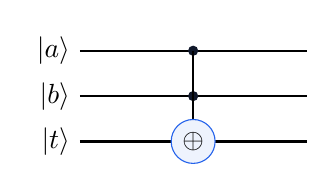
\begin{tikzpicture}[baseline=-0.55ex,scale=.72]
  \foreach \y/\n in {.8/a,0/b,-.8/t} {
    \draw[thick] (0,\y)--(4,\y);
    \node[left] at (0,\y) {$\ket{\n}$};
  }
  \fill[QpuNavy] (2,.8) circle (.09);
  \fill[QpuNavy] (2,0) circle (.09);
  \draw[thick] (2,.8)--(2,-.8);
  \node[draw=QpuBlue,fill=QpuBlue!8,circle,inner sep=2pt,font=\bfseries] at (2,-.8) {$\oplus$};
\end{tikzpicture}}

\newcommand{\SwapSegment}{%
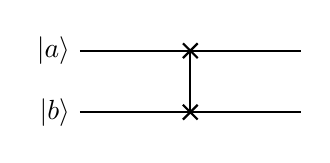
\begin{tikzpicture}[baseline=-0.55ex,scale=.78]
  \draw[thick] (0,.5)--(3.6,.5);
  \draw[thick] (0,-.5)--(3.6,-.5);
  \node[left] at (0,.5) {$\ket{a}$};
  \node[left] at (0,-.5) {$\ket{b}$};
  \draw[thick] (1.68,.38)--(1.92,.62) (1.68,.62)--(1.92,.38);
  \draw[thick] (1.68,-.38)--(1.92,-.62) (1.68,-.62)--(1.92,-.38);
  \draw[thick] (1.8,.5)--(1.8,-.5);
\end{tikzpicture}}

\newcommand{\MeasureSegment}{%
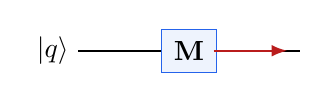
\begin{tikzpicture}[baseline=-0.55ex,scale=.78]
  \draw[thick] (0,0)--(3.6,0);
  \node[left] at (0,0) {$\ket{q}$};
  \node[draw=QpuBlue,fill=QpuBlue!8,minimum width=.7cm,minimum height=.55cm,font=\bfseries] at (1.8,0) {M};
  \draw[-{Latex[length=2mm]},QpuRed,thick] (2.2,0)--(3.4,0);
\end{tikzpicture}}

\newcommand{\GateHeading}[3]{%
\subsection{#1 (\code{#2})}
\begin{center}#3\end{center}}

\begin{document}

\begin{titlepage}
\pagecolor{QpuPaper}
\centering
\vspace*{1.25in}
{\Huge\bfseries\color{QpuNavy} QPU Static Circuit Compiler\par}
\vspace{0.2in}
{\LARGE\color{QpuBlue} Complete Protocol, Gate, and Truth-Table Reference\par}
\vspace{0.55in}
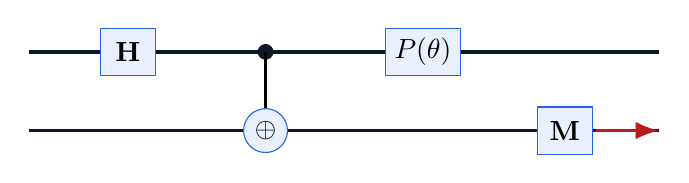
\begin{tikzpicture}
  \draw[very thick,QpuNavy] (0,1)--(8,1);
  \draw[very thick,QpuNavy] (0,0)--(8,0);
  \node[draw=QpuBlue,fill=QpuBlue!10,minimum width=.7cm,minimum height=.6cm,font=\bfseries] at (1.25,1) {H};
  \fill[QpuNavy] (3,1) circle (.1);
  \draw[very thick] (3,1)--(3,0);
  \node[draw=QpuBlue,fill=QpuBlue!10,circle,inner sep=2pt] at (3,0) {$\oplus$};
  \node[draw=QpuBlue,fill=QpuBlue!10,minimum width=.8cm,minimum height=.6cm,font=\bfseries] at (5,1) {$P(\theta)$};
  \node[draw=QpuBlue,fill=QpuBlue!10,minimum width=.7cm,minimum height=.6cm,font=\bfseries] at (6.8,0) {M};
  \draw[-{Latex[length=3mm]},QpuRed,very thick] (7.2,0)--(8,0);
\end{tikzpicture}
\vfill
{\large Bailey Forbes\par}
{\large September 13, 2026\par}
\vspace{0.35in}
\begin{minipage}{0.82\textwidth}
\small\color{QpuNavy}
This guide is derived from the current TypeScript AST parser, gate registry,
compiler, simulator, and truth-table implementation. It distinguishes syntax
that produces executable circuit gates from compatibility syntax that is only
recorded in the compiler log.
\end{minipage}
\vfill
\end{titlepage}
\nopagecolor

\tableofcontents
\newpage

\section{Scope and execution model}

The compiler turns a plain-text \code{.qpucir} protocol into one flat sequence
of circuit gates:
\[
\text{protocol source}\longrightarrow
\text{logical lines}\longrightarrow
\text{AST commands}\longrightarrow
\text{scoped tokens}\longrightarrow
\text{gates}\longrightarrow
\text{state-vector simulation}.
\]
Child processes are expanded at compile time. The UI and simulator therefore
see the same ordered gate list even when the source contains nested processes.

\subsection{Three levels of support}

\begin{tabularx}{\textwidth}{>{\bfseries}l X}
\toprule
Status & Meaning\\
\midrule
\implemented & The AST accepts the command and the compiler emits behavior
that the simulator executes.\\
\parsedonly & The AST accepts the command and preserves it in parsed output or
the compiler log, but no visual/simulator operation is emitted yet.\\
\internal & The compiler may emit the operation itself, but protocol source
cannot name it directly. \code{RESET} is the important example.\\
\bottomrule
\end{tabularx}

\subsection{Current AST command inventory}

\begin{longtable}{>{\ttfamily}p{0.24\textwidth}p{0.18\textwidth}p{0.48\textwidth}}
\toprule
\normalfont\bfseries Command & \bfseries Status & \bfseries Purpose\\
\midrule
\endhead
X, Y, Z, H, S, T, PHASE & \implemented & Single-qubit matrix operations.\\
CNOT, CCNOT, CZ, CY, SWAP & \implemented & Controlled and two-wire primitive operations.\\
NOT, AND, NAND, OR, XOR & \implemented & Derived logical target mutations.\\
MEASURE & \implemented & Measure one named wire or all known wires.\\
SET, CREATETOKEN & \implemented & Initialize/alias tokens and reserve wires.\\
RUNCHILD, CALL & \implemented & Expand a catalog/library child process.\\
RETURNVALS, ACCEPTVALS & \implemented & Bind child and process outputs.\\
MAIN-PROCESS, INCREASECYCLE & \implemented & Mark a process and flush cycle workspace.\\
FREE, DELETETOKEN, DECLARECHILD & \parsedonly & Lifetime/declaration hints; currently logged.\\
JOIN, SPLIT & \parsedonly & Register-memory compatibility syntax.\\
COMPILEPROCESS, MASTERVAL & \parsedonly & Process-control compatibility syntax.\\
\code{SAVE_STATE}, \code{LOAD_STATE} & \parsedonly & Checkpoint compatibility syntax.\\
\bottomrule
\end{longtable}

\textbf{Not source syntax:} \code{RESET} exists in the gate registry, but it is
not in the parser's supported-operation list. Write \code{SET wire 0p};
the compiler schedules internal \code{RESET} gates for zeroed workspace.

\section{Lexical and file syntax}

\subsection{Logical lines, whitespace, and case}

Commands and flags are case-insensitive and are separated by whitespace.
Token names retain their spelling. CRLF and LF line endings are accepted.
A physical line ending \emph{exactly} in a backslash joins to the next line:

\begin{lstlisting}
PARAMS: A:state B:state \
        Cin:state
CCNOT -I A B \
      -O Carry
\end{lstlisting}

The continuation backslash must be the final character; spaces after it prevent
continuation. Blank logical lines are discarded.

\subsection{Comments}

\begin{lstlisting}
# Whole-line or trailing hash comment
H -I Q:0 -O Q:0  # prepare |+>

/* A block comment may span logical lines. */
PHASE=pi/2 -I Q:0 -O Q:0
\end{lstlisting}

Continuation joining happens before comments are removed. Hash comments run to
the end of a logical line. C-style block comments use \code{/*} and \code{*/}.

\subsection{Protocol header}

\begin{lstlisting}
PARAMS: A:state B:state Theta:float Count:int

MAIN-PROCESS Example
\end{lstlisting}

\code{PARAMS:} is recognized only when it is the first non-comment logical
line. Each whitespace-separated entry containing a colon becomes
\code{name:type}. The parser does not restrict the type string:
\begin{itemize}
  \item \code{state} entries become user-facing circuit inputs and truth-table
  input columns;
  \item \code{int} and \code{float} entries are retained but excluded from
  user-facing qubit controls;
  \item other type names are retained as written.
\end{itemize}
The first \code{MAIN-PROCESS name} supplies the process name. If none exists,
the AST uses \code{InlineProcess}.

\subsection{Token references, cycles, and constants}

\begin{tabularx}{\textwidth}{>{\ttfamily}l X}
\toprule
\normalfont\bfseries Form & \bfseries Meaning\\
\midrule
Q & Bare symbolic token.\\
\$Q & Parameter/alias spelling; the leading dollar is removed during address
resolution.\\
Q:3 & Cycle/bit suffix; everything from the first colon is removed for the
current visual wire mapping. Thus \code{Q:0} and \code{Q:7} map to \code{Q}.\\
0p & Computational basis state $\ket{0}=[1,0]^T$.\\
1p & Computational basis state $\ket{1}=[0,1]^T$.\\
sp & Equal superposition $\ket{+}=(\ket{0}+\ket{1})/\sqrt2$.\\
0p\_dimN, 1p\_dimN, sp\_dimN & Also recognized as constants for an integer
\code{N}; the current compiler uses the same one-qubit initialization behavior.\\
\bottomrule
\end{tabularx}

Constants are case-insensitive and shared by canonical constant name. Numeric
workspace names passed to a child are scoped to the parent workspace; other
child-local names are scoped per invocation.

\subsection{Flags and argument boundaries}

Gate rows use \code{-I} and \code{-O}:
\begin{lstlisting}
GATE -I input1 input2 -O output
\end{lstlisting}
Each list ends at the next token beginning with a hyphen. Flags are
case-insensitive. Positional \code{args} still contain every token after the
opcode, including flags. The AST also records \code{-$R} as
\code{noParameterSubstitution}; the current compiler does not act on that flag.

\begin{lstlisting}
PHASE=pi/4 -I Q -O Q -$R
\end{lstlisting}

\subsection{Gate arity}

\begin{center}
\begin{tabular}{lll}
\toprule
Gate family & Required \code{-I} count & Required \code{-O} count\\
\midrule
X, Y, Z, H, S, T, PHASE, NOT & 1 & 1\\
CNOT, CZ, CY & 1 & 1\\
CCNOT, AND, NAND, OR, XOR & 2 & 1\\
SWAP & 2 & 2\\
MEASURE & 0 or 1 & 0\\
\bottomrule
\end{tabular}
\end{center}

All counts are exact except \code{MEASURE}. For ordinary single-qubit gates,
name the same wire in \code{-I} and \code{-O}. The output is the mutated target;
for controlled gates, \code{-I} contains controls.

\section{Quantum state mathematics}

One qubit is a normalized complex vector:
\[
\ket{\psi}=\alpha\ket0+\beta\ket1
=\begin{bmatrix}\alpha\\\beta\end{bmatrix},
\qquad |\alpha|^2+|\beta|^2=1.
\]
A gate $U$ acts linearly: $\ket{\psi'}=U\ket{\psi}$. A valid closed-system
gate is unitary, $U^\dagger U=I$, so normalization is preserved.

For $n$ qubits, basis states are tensor products and the state has $2^n$
amplitudes:
\[
\ket{\Psi}=\sum_{x=0}^{2^n-1} a_x\ket{x},\qquad
\sum_x |a_x|^2=1,\qquad
\ket{AB}=\ket A\otimes\ket B.
\]
The simulator stores this state vector directly. A controlled operation applies
its target matrix only to basis components whose controls satisfy its predicate.

\subsection{Measurement}

For a measured qubit $q$,
\[
P(q=1)=\sum_{x:\,x_q=1}|a_x|^2,\qquad
P(q=0)=1-P(q=1).
\]
After sampling $b\in\{0,1\}$, incompatible amplitudes are set to zero and the
remaining branch is renormalized by $1/\sqrt{P(q=b)}$. Measurement is therefore
not a unitary matrix operation.

\subsection{Truth tables versus amplitudes}

A classical truth table describes deterministic basis-state behavior. It
cannot show relative phase or interference. Consequently, the tables below
compare basis mappings, while matrices and state equations describe the full
quantum action. In companion \code{.qpuio} tables, cells are \code{0p},
\code{1p}, or \code{sp}; an expected output \code{sp} is treated as
``don't care'' during measured-output comparison.

\section{Single-qubit primitive gates}

\GateHeading{Pauli X}{X}{\GateSegment{X}}

\[
X=\begin{bmatrix}0&1\\1&0\end{bmatrix},\quad
X\ket0=\ket1,\quad X\ket1=\ket0,\quad
X(\alpha\ket0+\beta\ket1)=\beta\ket0+\alpha\ket1.
\]
\begin{lstlisting}
X -I Q:0 -O Q:0
\end{lstlisting}
\begin{center}
\begin{tabular}{ccc}\toprule Input & Classical comparison & Output\\\midrule
0 & NOT 0 & 1\\
1 & NOT 1 & 0\\\bottomrule\end{tabular}
\end{center}

\GateHeading{Pauli Y}{Y}{\GateSegment{Y}}

\[
Y=\begin{bmatrix}0&-i\\i&0\end{bmatrix},\quad
Y\ket0=i\ket1,\quad Y\ket1=-i\ket0.
\]
It flips the basis value like X but adds phases that become observable through
later interference.
\begin{lstlisting}
Y -I Q -O Q
\end{lstlisting}
\begin{center}
\begin{tabular}{ccc}\toprule Input & Measured bit & Quantum output\\\midrule
0 & 1 & $i\ket1$\\
1 & 0 & $-i\ket0$\\\bottomrule\end{tabular}
\end{center}

\GateHeading{Pauli Z}{Z}{\GateSegment{Z}}

\[
Z=\begin{bmatrix}1&0\\0&-1\end{bmatrix},\quad
Z\ket0=\ket0,\quad Z\ket1=-\ket1.
\]
Z does not change a computational-basis measurement, but it changes relative
phase. For example, $Z\ket+=\ket-=(\ket0-\ket1)/\sqrt2$.
\begin{lstlisting}
Z -I Q -O Q
\end{lstlisting}
\begin{center}
\begin{tabular}{ccc}\toprule Input & Classical bit & Quantum output\\\midrule
0 & 0 & $\ket0$\\
1 & 1 & $-\ket1$\\\bottomrule\end{tabular}
\end{center}

\GateHeading{Hadamard}{H}{\GateSegment{H}}

\[
H=\frac1{\sqrt2}\begin{bmatrix}1&1\\1&-1\end{bmatrix},\quad
H\ket0=\ket+,\quad H\ket1=\ket-.
\]
\begin{lstlisting}
SET Q 0p
H -I Q -O Q
MEASURE -I Q
\end{lstlisting}
\begin{center}
\begin{tabular}{ccc}\toprule Input & Measurement distribution & State before measurement\\\midrule
0 & 50\% 0, 50\% 1 & $(\ket0+\ket1)/\sqrt2$\\
1 & 50\% 0, 50\% 1 & $(\ket0-\ket1)/\sqrt2$\\\bottomrule\end{tabular}
\end{center}
Equal classical probabilities hide the relative minus sign responsible for
interference.

\GateHeading{S phase}{S}{\GateSegment{S}}

\[
S=P(\pi/2)=\begin{bmatrix}1&0\\0&i\end{bmatrix},\qquad
S\ket1=i\ket1,\qquad S^2=Z.
\]
\begin{lstlisting}
S -I Q -O Q
\end{lstlisting}
\begin{center}
\begin{tabular}{ccc}\toprule Input & Measured bit & Quantum output\\\midrule
0 & 0 & $\ket0$\\
1 & 1 & $i\ket1$\\\bottomrule\end{tabular}
\end{center}

\GateHeading{T phase}{T}{\GateSegment{T}}

\[
T=P(\pi/4)=\begin{bmatrix}1&0\\0&e^{i\pi/4}\end{bmatrix},\qquad
T^2=S,\qquad T^4=Z.
\]
\begin{lstlisting}
T -I Q -O Q
\end{lstlisting}
\begin{center}
\begin{tabular}{ccc}\toprule Input & Measured bit & Quantum output\\\midrule
0 & 0 & $\ket0$\\
1 & 1 & $e^{i\pi/4}\ket1$\\\bottomrule\end{tabular}
\end{center}

\GateHeading{Arbitrary phase}{PHASE}{\GateSegment{$P(\theta)$}}

\[
P(\theta)=\begin{bmatrix}1&0\\0&e^{i\theta}\end{bmatrix},\qquad
\alpha\ket0+\beta\ket1\mapsto
\alpha\ket0+\beta e^{i\theta}\ket1.
\]
The angle is embedded in the opcode:
\begin{lstlisting}
PHASE=1.5708 -I Q -O Q     # radians
PHASE=3/2 -I Q -O Q        # rational radians
PHASE=90d -I Q -O Q        # degrees
PHASE=45/2d -I Q -O Q      # rational degrees
PHASE=pi -I Q -O Q
PHASE=-11pi/6 -I Q -O Q
PHASE=2*pi/3 -I Q -O Q
BPHASE=pi/4 -I Q -O Q      # P(-pi/4)
\end{lstlisting}
Accepted numeric atoms include signed integers, decimals, leading-dot decimals,
and one optional rational denominator. Pi notation accepts an optional sign,
an integer coefficient, an optional \code{*}, and an optional positive integer
denominator. A zero denominator and malformed angle raise an error.

\begin{center}
\begin{tabular}{ccc}\toprule Input & Measured bit & Quantum output\\\midrule
0 & 0 & $\ket0$\\
1 & 1 & $e^{i\theta}\ket1$\\\bottomrule\end{tabular}
\end{center}

\subsection{Backward-prefix syntax}

The AST recognizes a leading \code{B} before any registered primitive gate
name, for example \code{BX}, \code{BH}, \code{BCNOT}, or \code{BSWAP}, and
sets \code{reverse=true}. Only \code{BPHASE=angle} currently changes emitted
behavior: the compiler negates the phase angle. For every other gate the flag
is presently metadata only. Many gates are self-inverse ($X,H,\mathrm{CNOT},
\mathrm{CCNOT},\mathrm{CZ},\mathrm{SWAP}$), but S, T, Y, and CY inverses are
\emph{not} synthesized from the reverse flag. Do not rely on those B-prefixed
forms for inverse execution.

\section{Controlled and two-qubit primitive gates}

\GateHeading{Controlled NOT}{CNOT}{\ControlledSegment{$\oplus$}}

\[
\ket{c,t}\longmapsto\ket{c,t\oplus c}.
\]
\begin{lstlisting}
CNOT -I Control -O Target
\end{lstlisting}
\begin{center}
\begin{tabular}{cc|cc}\toprule $c$&$t$&$c'$&$t'$\\\midrule
0&0&0&0\\0&1&0&1\\1&0&1&1\\1&1&1&0\\\bottomrule
\end{tabular}
\end{center}
CNOT is a reversible embedding of XOR because it preserves the control.

\GateHeading{Doubly controlled NOT / Toffoli}{CCNOT}{\DoubleControlledSegment}

\[
\ket{a,b,t}\longmapsto\ket{a,b,t\oplus(a\land b)}.
\]
\begin{lstlisting}
CCNOT -I A B -O Target
\end{lstlisting}
\begin{center}
\begin{tabular}{ccc|ccc}\toprule $a$&$b$&$t$&$a'$&$b'$&$t'$\\\midrule
0&0&0&0&0&0\\0&0&1&0&0&1\\
0&1&0&0&1&0\\0&1&1&0&1&1\\
1&0&0&1&0&0\\1&0&1&1&0&1\\
1&1&0&1&1&1\\1&1&1&1&1&0\\\bottomrule
\end{tabular}
\end{center}
With a target initialized to zero, Toffoli computes classical AND reversibly.

\GateHeading{Controlled Z}{CZ}{\ControlledSegment{Z}}

\[
\mathrm{CZ}\ket{c,t}=(-1)^{ct}\ket{c,t},\qquad
\mathrm{CZ}=\operatorname{diag}(1,1,1,-1).
\]
\begin{lstlisting}
CZ -I Control -O Target
\end{lstlisting}
\begin{center}
\begin{tabular}{cc|cc}\toprule Input & Measured output & Amplitude multiplier & State\\\midrule
00&00&$+1$&$\ket{00}$\\01&01&$+1$&$\ket{01}$\\
10&10&$+1$&$\ket{10}$\\11&11&$-1$&$-\ket{11}$\\\bottomrule
\end{tabular}
\end{center}
The classical columns are unchanged; the quantum phase is the operation.

\GateHeading{Controlled Y}{CY}{\ControlledSegment{Y}}

\[
\ket{0,t}\mapsto\ket{0,t},\quad
\ket{1,0}\mapsto i\ket{1,1},\quad
\ket{1,1}\mapsto-i\ket{1,0}.
\]
\begin{lstlisting}
CY -I Control -O Target
\end{lstlisting}
\begin{center}
\begin{tabular}{cc|cc|c}\toprule $c$&$t$&$c'$&$t'$&Quantum phase\\\midrule
0&0&0&0&$+1$\\0&1&0&1&$+1$\\
1&0&1&1&$i$\\1&1&1&0&$-i$\\\bottomrule
\end{tabular}
\end{center}

\GateHeading{Swap}{SWAP}{\SwapSegment}

\[
\mathrm{SWAP}\ket{a,b}=\ket{b,a}.
\]
\begin{lstlisting}
SWAP -I A B -O A B
\end{lstlisting}
The two output tokens are mandatory and must resolve to the same two wires, in
the same order, as the inputs.
\begin{center}
\begin{tabular}{cc|cc}\toprule $a$&$b$&$a'$&$b'$\\\midrule
0&0&0&0\\0&1&1&0\\1&0&0&1\\1&1&1&1\\\bottomrule
\end{tabular}
\end{center}

\section{Derived logical gates}

Derived gates are direct AST operations implemented as reversible target
mutations. Inputs are preserved. If target $t$ starts in zero, AND/OR/XOR
write the familiar classical function. If it does not, the true behavior is
the XOR embedding shown below.

\GateHeading{Logical NOT}{NOT}{\GateSegment{$\neg$}}

\[
t'\;=\;t\oplus1.
\]
\begin{lstlisting}
NOT -I Target -O Target
\end{lstlisting}
\begin{center}
\begin{tabular}{c|c}\toprule $t$&$t'$\\\midrule0&1\\1&0\\\bottomrule\end{tabular}
\end{center}
The current gate implementation mutates the output target. Use the same token
for input and output; a distinct input token is not copied.

\GateHeading{Reversible AND}{AND}{\DoubleControlledSegment}

\[
t'=t\oplus(a\land b).
\]
\begin{lstlisting}
SET Out 0p
AND -I A B -O Out
\end{lstlisting}
\begin{center}
\begin{tabular}{cc|c|c}\toprule $a$&$b$&$t=0$&$t'=a\land b$\\\midrule
0&0&0&0\\0&1&0&0\\1&0&0&0\\1&1&0&1\\\bottomrule
\end{tabular}
\end{center}

\GateHeading{Reversible NAND}{NAND}{\DoubleControlledSegment}

\[
t'=t\oplus(a\land b)\oplus1.
\]
\begin{lstlisting}
SET Out 0p
NAND -I A B -O Out
\end{lstlisting}
\begin{center}
\begin{tabular}{cc|c|c}\toprule $a$&$b$&$t=0$&$t'=\neg(a\land b)$\\\midrule
0&0&0&1\\0&1&0&1\\1&0&0&1\\1&1&0&0\\\bottomrule
\end{tabular}
\end{center}

\GateHeading{Reversible OR}{OR}{\DoubleControlledSegment}

\[
t'=t\oplus(a\lor b).
\]
\begin{lstlisting}
SET Out 0p
OR -I A B -O Out
\end{lstlisting}
\begin{center}
\begin{tabular}{cc|c|c}\toprule $a$&$b$&$t=0$&$t'=a\lor b$\\\midrule
0&0&0&0\\0&1&0&1\\1&0&0&1\\1&1&0&1\\\bottomrule
\end{tabular}
\end{center}
For bits, $a\lor b=a\oplus b\oplus(a\land b)$.

\GateHeading{Reversible XOR}{XOR}{\DoubleControlledSegment}

\[
t'=t\oplus a\oplus b.
\]
\begin{lstlisting}
SET Out 0p
XOR -I A B -O Out
\end{lstlisting}
\begin{center}
\begin{tabular}{cc|c|c}\toprule $a$&$b$&$t=0$&$t'=a\oplus b$\\\midrule
0&0&0&0\\0&1&0&1\\1&0&0&1\\1&1&0&0\\\bottomrule
\end{tabular}
\end{center}

\section{Measurement gate}

\GateHeading{Measurement}{MEASURE}{\MeasureSegment}

\begin{lstlisting}
MEASURE -I Q     # exactly one named wire
MEASURE          # every wire known at this point
\end{lstlisting}
\code{MEASURE} takes no \code{-O}. Repeated one-wire commands are useful when
only declared returns should become classical. A bare command emits one
measurement operation per currently allocated wire.

\begin{center}
\begin{tabular}{c|c|c}\toprule State & Outcome probabilities & Collapsed state\\\midrule
$\ket0$ & $P(0)=1$ & $\ket0$\\
$\ket1$ & $P(1)=1$ & $\ket1$\\
$\alpha\ket0+\beta\ket1$ & $P(0)=|\alpha|^2$, $P(1)=|\beta|^2$ &
$\ket0$ or $\ket1$\\\bottomrule
\end{tabular}
\end{center}

\section{State, token, and cycle commands}

\subsection{\code{SET} --- initialize or alias (\implemented)}

\begin{lstlisting}
SET Q 0p
SET Q 1p
SET Q sp
SET Local $Parameter
\end{lstlisting}
\code{SET target value} requires a positional value. A constant schedules or
emits initialization: zero, X from zero, or H from zero. A nonconstant value
makes the target an alias of that source. A \code{state} parameter's constant
SET is treated as a runtime default, allowing the UI or truth-table runner to
supply its actual start state.

\subsection{\code{CREATETOKEN} --- reserve wires (\implemented)}

\begin{lstlisting}
CREATETOKEN -I Sum Carry Workspace
\end{lstlisting}
Every \code{-I} token immediately claims a stable wire index. No \code{-O} is
used. This is useful for declared outputs before their first gate.

\subsection{\code{DELETETOKEN} and \code{FREE} --- lifetime hints (\parsedonly)}

\begin{lstlisting}
DELETETOKEN -I Workspace
FREE -I ScratchA ScratchB
\end{lstlisting}
Both commands are accepted and logged. They do not currently remove, reset, or
reuse a wire; later compaction removes symbolic registers that never participate
in an emitted gate or exposed parameter.

\subsection{\code{INCREASECYCLE} --- cycle boundary (\implemented)}

\begin{lstlisting}
INCREASECYCLE
\end{lstlisting}
The compiler flushes pending zero-initializations into an internal batched
\code{RESET}, increments the cycle counter, and prepares workspace for following
operations. Cycle suffixes on tokens do not create separate visual wires.

\subsection{\code{JOIN} and \code{SPLIT} (\parsedonly)}

\begin{lstlisting}
JOIN -I A B -O AB
SPLIT AB A 2
\end{lstlisting}
The intended mathematical model for a clean join is
$\ket{AB}=\ket A\otimes\ket B$. A split into independent pure states is only
possible when the composite state factors. The current compiler merely logs
these rows: no tensor-product allocation, extraction, gate, or alias is emitted.
Because these are non-gate commands, the parser does not enforce their arity.

\section{Process composition and return values}

\subsection{\code{MAIN-PROCESS} (\implemented)}

\begin{lstlisting}
MAIN-PROCESS FullAdder
\end{lstlisting}
This marks the process body and supplies its catalog/library name. Compilation
already begins from the parsed process, so the row itself emits no gate.

\subsection{\code{DECLARECHILD} (\parsedonly)}

\begin{lstlisting}
DECLARECHILD SingleBitFullAdder
\end{lstlisting}
The declaration is logged. It does not load inline source. Child bodies must
exist in the external \code{librarySources} catalog when called.

\subsection{\code{RUNCHILD} and \code{CALL} (\implemented)}

\begin{lstlisting}
RUNCHILD SingleBitFullAdder \
  -I A B Cin \
  -O Carry Sum

CALL SingleBitFullAdder -I A B Cin -O Carry Sum
\end{lstlisting}
The two commands currently have the same expansion behavior. The first
positional argument is the child process name. Inputs bind by PARAMS order;
outputs bind by the child's RETURNVALS order. Before expansion, each bound
parent output is zero-prepared once. Child-local names receive a unique scope.

\subsection{\code{RETURNVALS} (\implemented)}

\begin{lstlisting}
RETURNVALS Carry Sum
\end{lstlisting}
Positional tokens define the process's ordered public outputs. They determine
child output binding, truth-table output columns, and the UI's preferred
logical width. Do not use \code{-I} or \code{-O} here: flags would be retained
as positional return tokens.

\subsection{\code{ACCEPTVALS} (\implemented)}

\begin{lstlisting}
CALL Child -I A B
ACCEPTVALS LocalCarry LocalSum
\end{lstlisting}
Each positional local token aliases the corresponding value from the most
recent child return list. Direct \code{-O} binding on RUNCHILD/CALL is clearer
when output names are known.

\subsection{Nested full-adder example}

\begin{lstlisting}
# child.qpucir
PARAMS: A:state B:state Cin:state
MAIN-PROCESS ChildAdder
CREATETOKEN -I Carry Sum
SET Carry 0p
SET Sum 0p
XOR   -I A B   -O Sum
CNOT -I Cin   -O Sum
CCNOT -I A B   -O Carry
CCNOT -I A Cin -O Carry
CCNOT -I B Cin -O Carry
RETURNVALS Carry Sum
\end{lstlisting}

\begin{lstlisting}
# parent.qpucir
PARAMS: A:state B:state Cin:state
MAIN-PROCESS Parent
CREATETOKEN -I Cout Result
RUNCHILD ChildAdder -I A B Cin -O Cout Result
MEASURE -I Cout
MEASURE -I Result
RETURNVALS Cout Result
\end{lstlisting}

For basis inputs, the full-adder equations are
\[
\mathrm{Sum}=A\oplus B\oplus C_{\mathrm{in}},\qquad
C_{\mathrm{out}}=(A\land B)\oplus(A\land C_{\mathrm{in}})
\oplus(B\land C_{\mathrm{in}}).
\]
\begin{center}
\begin{tabular}{ccc|cc}\toprule
$A$&$B$&$C_{\rm in}$&$C_{\rm out}$&Sum\\\midrule
0&0&0&0&0\\0&0&1&0&1\\0&1&0&0&1\\0&1&1&1&0\\
1&0&0&0&1\\1&0&1&1&0\\1&1&0&1&0\\1&1&1&1&1\\\bottomrule
\end{tabular}
\end{center}

\section{Accepted compatibility commands}

The following rows are valid AST commands but currently produce log entries
only. Their arguments are retained as whitespace-separated strings and their
arity is not validated.

\begin{longtable}{>{\ttfamily}p{0.22\textwidth}p{0.36\textwidth}p{0.32\textwidth}}
\toprule
\normalfont\bfseries Command & \bfseries Example & \bfseries Current effect\\
\midrule
\endhead
COMPILEPROCESS & \code{COMPILEPROCESS Child} & Logs process-control text; does
not load or compile a child. Use RUNCHILD/CALL with library source.\\
MASTERVAL & \code{MASTERVAL Result} & Logs a final/master-value marker; does
not alter RETURNVALS.\\
\code{SAVE_STATE} & \code{SAVE_STATE checkpointA} & Logs a checkpoint request; no
state snapshot is created.\\
\code{LOAD_STATE} & \code{LOAD_STATE checkpointA} & Logs a restore request; no state
is changed.\\
\bottomrule
\end{longtable}

\section{Truth-table companion syntax}

Truth tables are metadata paired to a process; they are not \code{.qpucir} AST
commands. A text \code{.qpuio} file may use spaces or commas:

\begin{lstlisting}
MAIN-PROCESS: HalfAdder
INPUTS: A B
OUTPUTS: Carry Sum
# A B Carry Sum
0 0p 0p 0p 0p
1 0p 1p 0p 1p
2 1p 0p 0p 1p
3 1p 1p 1p 0p
\end{lstlisting}

\begin{itemize}
  \item \code{MAIN-PROCESS: name} and a column row beginning with \texttt{\#}
  are required.
  \item Explicit \code{INPUTS:} and \code{OUTPUTS:} remove ambiguity. Without
  them, the parser can use matching PARAMS/RETURNVALS from the protocol.
  \item Data rows begin at index 0 and must be sequential.
  \item Every row must match the header width and every cell must be
  \code{0p}, \code{1p}, or \code{sp}.
  \item Comma-separated headers and rows are also accepted.
  \item Partial tables may list fewer than $2^n$ distinct input patterns, but
  not zero rows, duplicates, or more than $2^n$ rows.
\end{itemize}

The JSON envelope form is:
\begin{lstlisting}[language={}]
{
  "format": "qpuio",
  "version": 1,
  "processName": "HalfAdder",
  "inputColumns": ["A", "B"],
  "outputColumns": ["Carry", "Sum"],
  "rows": [
    ["0p", "0p", "0p", "0p"],
    ["0p", "1p", "0p", "1p"],
    ["1p", "0p", "0p", "1p"],
    ["1p", "1p", "1p", "0p"]
  ]
}
\end{lstlisting}

The table runner initializes PARAMS by column order, executes the circuit,
measures RETURNVALS, and compares those bits only. An expected output
\code{sp} accepts either measured bit; an input \code{sp} initializes an equal
superposition before execution.

\section{Complete worked protocol}

\begin{lstlisting}
PARAMS: A:state B:state Theta:float

MAIN-PROCESS BellAndLogic
CREATETOKEN -I Q0 Q1 AndOut

SET Q0 $A
SET Q1 $B
SET AndOut 0p

# Quantum segment
H -I Q0 -O Q0
CNOT -I Q0 -O Q1
PHASE=pi/4 -I Q1 -O Q1

# Basis-state comparison output
AND -I A B -O AndOut

MEASURE -I Q0
MEASURE -I Q1
MEASURE -I AndOut
RETURNVALS Q0 Q1 AndOut
\end{lstlisting}

Starting from $\ket{00}$, the H--CNOT segment prepares
\[
\ket{00}\xrightarrow{H\otimes I}
\frac{\ket{00}+\ket{10}}{\sqrt2}
\xrightarrow{\mathrm{CNOT}}
\frac{\ket{00}+\ket{11}}{\sqrt2}.
\]
The phase gate then produces
\[
\frac{\ket{00}+e^{i\pi/4}\ket{11}}{\sqrt2}.
\]
The two quantum measurements are correlated, while \code{AndOut} compares the
basis inputs through $A\land B$. A deterministic truth table can specify the
logic output, but repeated simulation is needed to characterize Bell-state
measurement probabilities.

\section{Compiler output and lowering details}

Compilation returns:
\begin{lstlisting}[language={}]
CompileResult {
  gates: CircuitGate[]
  qubitCount: number
  logicalQubitCount: number
  parsed: ParsedCommand[]
  log: string[]
  tokenMap: Record<string, number>
  processParams: ProcessParam[]
  returnValues: ReturnValue[]
}
\end{lstlisting}

Each parsed command records \code{op}, original \code{raw} text,
\code{inputs}, \code{outputs}, positional \code{args}, optional normalized
radian \code{phase}, \code{reverse}, and \code{noParameterSubstitution}.
Each emitted gate records \code{id}, \code{type}, ordered \code{step},
\code{targets}, \code{controls}, optional \code{phase}, and source text.

After child expansion, unused symbolic holes are compacted to dense qubit
indices. Internal RESET gates count for simulation but are filtered from the
visible circuit. UI logical width prefers RETURNVALS count, then exposed PARAMS
count, then physical simulator width.

\section{Error conditions and practical rules}

\begin{enumerate}
  \item Unknown opcodes fail with \code{Unknown command}. \code{RESET} is not a
  source opcode.
  \item Every AST gate except MEASURE requires \code{-I} and \code{-O}, then
  exact registry arity is checked.
  \item PHASE requires a valid nonzero-denominator angle after \code{=}.
  \item SWAP requires two matching input/output wires.
  \item RUNCHILD/CALL fails if the named process is absent from the library.
  \item SET fails when its positional value is missing.
  \item RETURNVALS order is semantically significant for child bindings and
  truth-table columns.
  \item Use the same input/output token for single-qubit gates.
  \item Initialize derived-gate targets deliberately; their operation is XOR
  into the existing target, not destructive assignment.
  \item Treat parsed-only commands as compatibility annotations until their
  runtime lowering is implemented.
\end{enumerate}

\section{Quick-reference grammar}

This is a practical description of the accepted surface language rather than a
separate parser generator grammar:
\begin{lstlisting}[language={}]
protocol     := [params-line] logical-line*
params-line  := "PARAMS:" (name ":" type)*
logical-line := command | comment | blank

command      := opcode argument*
opcode       := supported-command
             | primitive-gate
             | "B" primitive-gate
             | "PHASE=" angle
             | "BPHASE=" angle

gate-row     := opcode "-I" input+ "-O" output+ ["-$R"]
measure-row  := "MEASURE" ["-I" input]
set-row      := "SET" target value
process-row  := "MAIN-PROCESS" name
child-row    := ("RUNCHILD" | "CALL") name
                ["-I" argument*] ["-O" argument*]
returns-row  := "RETURNVALS" token*
accept-row   := "ACCEPTVALS" token*

token        := ["$"] name [":" suffix]
constant     := ("0p" | "1p" | "sp") ["_dim" integer]
angle        := rational
             | rational "d"
             | [sign] [integer ["*"]] "pi" ["/" integer]
\end{lstlisting}

\textbf{Parser detail:} \code{PHASE= pi/2} is joined into one opcode/value pair,
but \code{PHASE = pi/2} is not. Operations and flags are case-insensitive;
names, types, and positional values are otherwise retained.

\section{Operation checklist}

\begin{center}
\small
\begin{tabularx}{\textwidth}{>{\ttfamily}l X >{\ttfamily}l X}
\toprule
\normalfont\bfseries Item & \bfseries Covered in &
\normalfont\bfseries Item & \bfseries Covered in\\
\midrule
PARAMS: & Lexical syntax & MAIN-PROCESS & Process composition\\
X,Y,Z,H & Single-qubit gates & S,T,PHASE & Single-qubit gates\\
CNOT,CCNOT & Controlled gates & CZ,CY,SWAP & Controlled gates\\
NOT,AND,NAND & Derived gates & OR,XOR & Derived gates\\
MEASURE & Measurement & SET & State/token commands\\
CREATETOKEN & State/token commands & DELETETOKEN,FREE & State/token commands\\
INCREASECYCLE & State/token commands & JOIN,SPLIT & State/token commands\\
DECLARECHILD & Process composition & RUNCHILD,CALL & Process composition\\
RETURNVALS & Process composition & ACCEPTVALS & Process composition\\
COMPILEPROCESS & Compatibility & MASTERVAL & Compatibility\\
\code{SAVE_STATE} & Compatibility & \code{LOAD_STATE} & Compatibility\\
-I,-O,-\$R & Flags & B prefix & Single-qubit/reverse syntax\\
comments,\textbackslash & Lexical syntax & .qpuio & Truth-table syntax\\
\bottomrule
\end{tabularx}
\end{center}

\vfill
\begin{center}
\textcolor{CodeComment}{\small End of complete AST and circuit reference}
\end{center}

\end{document}
